\FloatBarrier
Licht hat einen Teilchen- und einen Wellencharakter. Diese sind die Grenzfälle der Quantenelektrodynamik. Für den Photoefekt ist nur die korpuskale Betrachnungsweise von Bedeutung. Bei dieser Betrachtung wird die Energie in Form von Lichtquanten durch den Raum transportiert.
Die Energie der Photonen tritt nur gequantelt auf. Wenn die Photonen auf ein Elektron treffen, so können diese ihre Energie an die Elektronen abgeben. Die Energie der Elektronen nach dem Stoß setzt sich wie folgt zusammen:
\begin{equation}
  E_{kin}= h\nu-A_k.
\label{eqn:energieE}
\end{equation}
$h$ ist dabei das Plancksche Wirkungsquantum und $\nu$ die Frequenz des Lichtes. $A_k$ beschreibt die Austrittsarbeit eines Elektrons welche von Material zu Material unterschiedlich ist. Zusätzlich ist $E_{kin}$ von der Energie abhängig welche die Elektronen im Material besaßen, dies kann jedoch vernachlässigt werden.
Der Gleichung ist zu entnehmen, dass die Energie der Elektronen abhängig von der Freqeuenz $\nu$ ist. Es gibt eine Grenzfrequenz, wenn die Energie des Photons kleiner ist als die Austritsarbeit, unter der keine Elektronen ausgelöst werden können. Die Intensität des eingestralten Lichtes hat nur einen Einfluss auf die Anzahl der ausgelösten Elektronen pro Zeit nicht aber auf die Energie. Mit der Fermi-Dirac-Statistik lässt sich eine Aussage über die Energieverteilung der Elektronen im Festkörper treffen. Die Energie der Elektronen kann demnach nur zwischen 0 und der Fermi-Energie liegen. Temperaturabhängig gibt es vereinzelt Elektronen deren Energie über der Fermi-Energie liegt.\\
Für den Photostrom gilt desweiteren:
\begin{equation*}
  h\nu+e_{0}U_{\text{b}} \geq A_A
\end{equation*}
$A_A$ ist die Austrittsabeit aus der Anode. Ist $A_A$ größer als $h\nu+e_0U_{\text{b}}$ so kann es, wie in Abbildung \ref{fig:500-6} zu sehen ist, zu einem negativen Strom kommen.



\begin{figure}
 \centering
 \begin{subfigure}{0.48\textwidth}
  \centering
  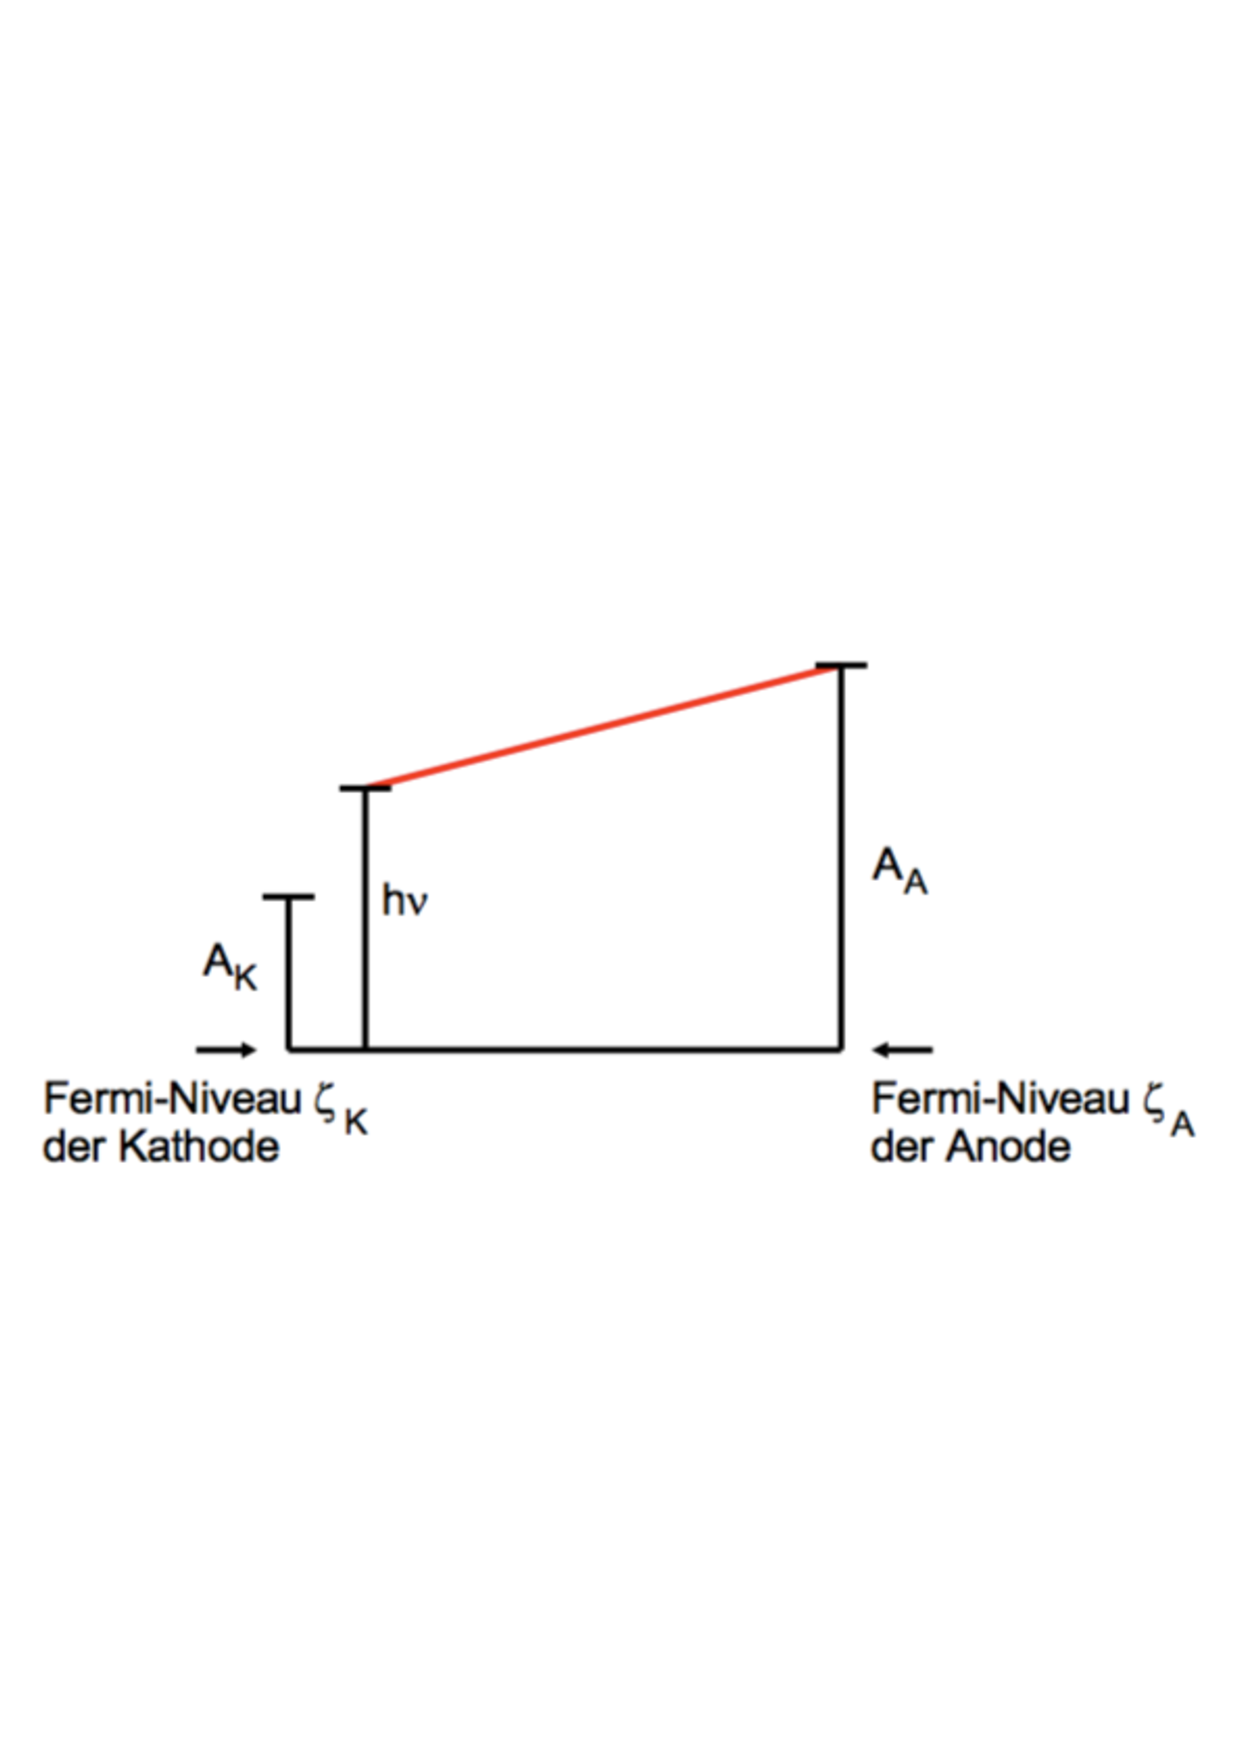
\includegraphics[width=1.2\textwidth]{500-6.pdf}
  \caption{Negativer Strom \cite{1}}
  \label{fig:500-6}
 \end{subfigure}
 \begin{subfigure}{0.48\textwidth}
  \centering
  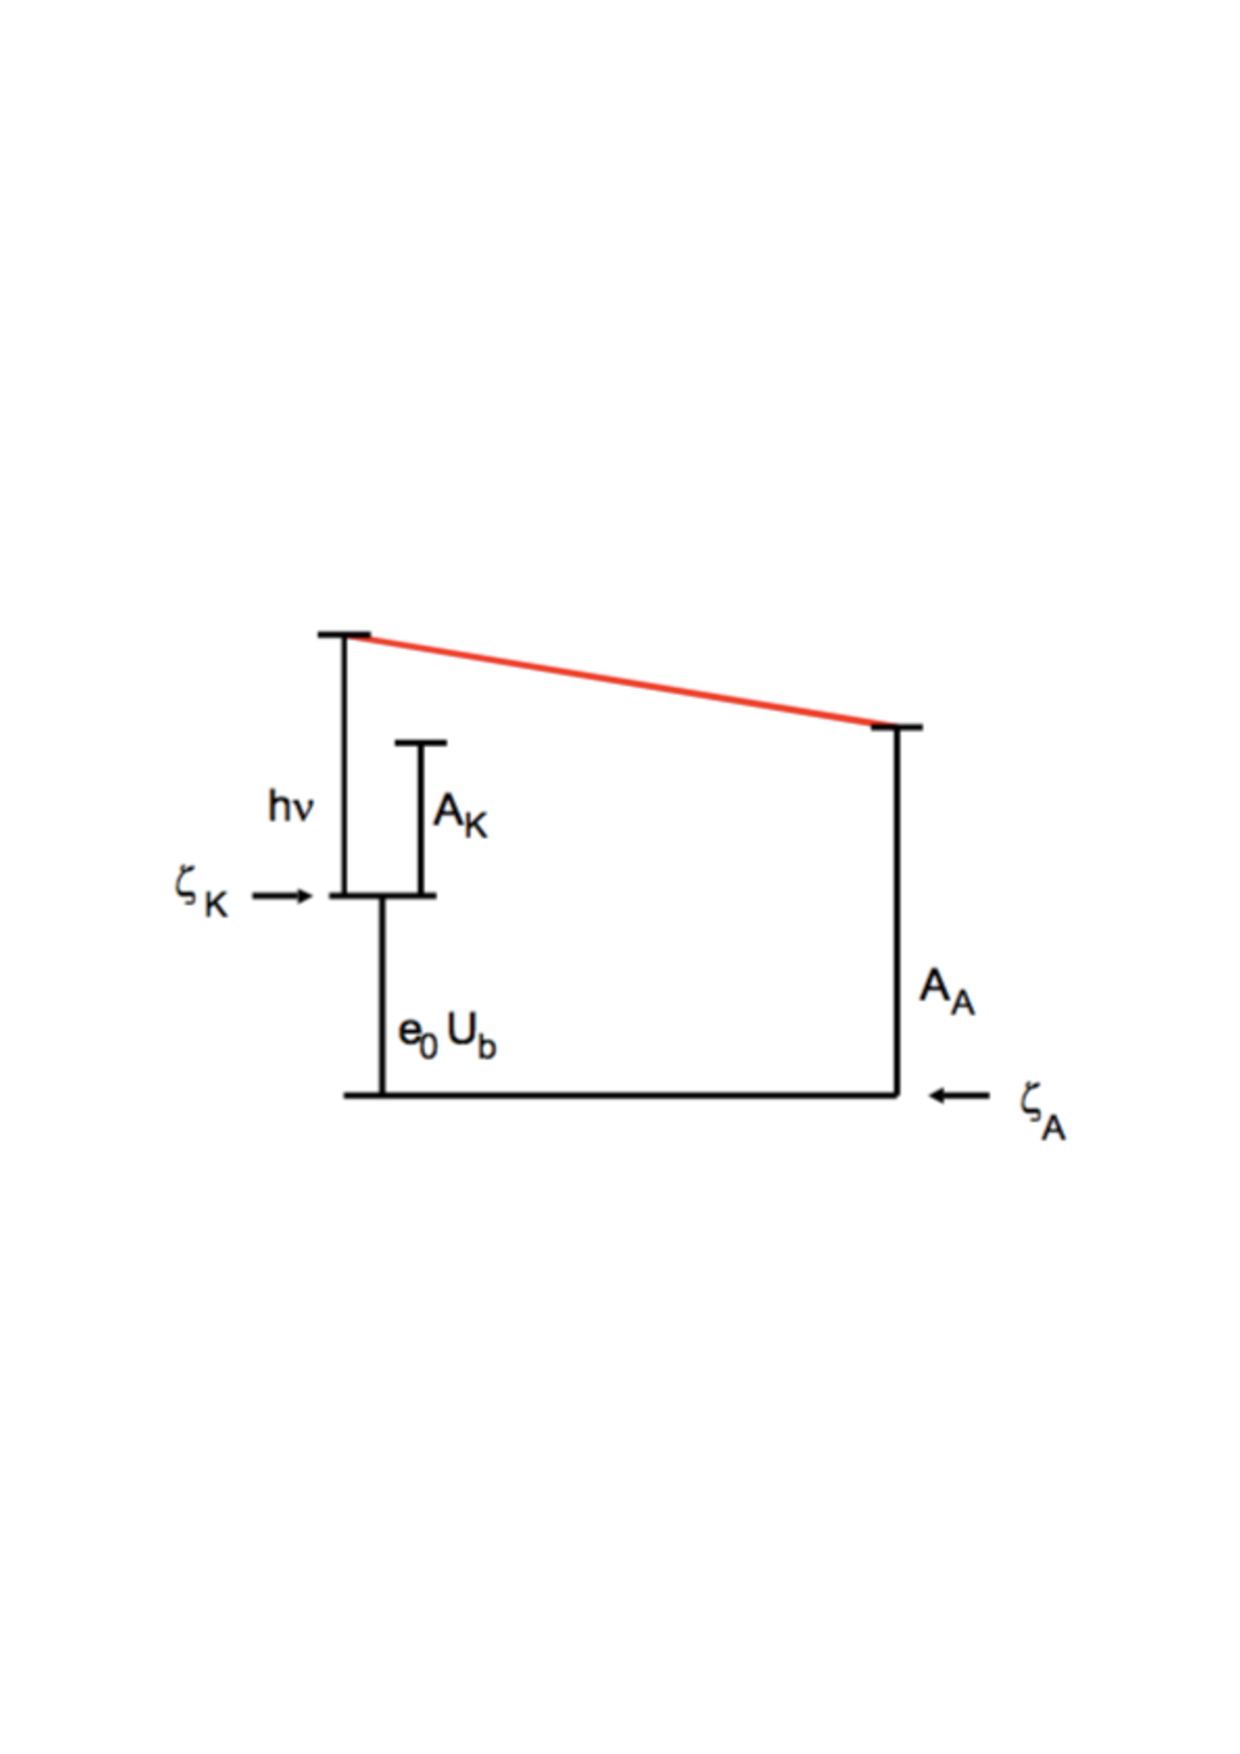
\includegraphics[width=0.8\textwidth]{500-7.pdf}
  \caption{Positiver Strom \cite{1}}
  \label{fig:500-7}
 \end{subfigure}
 \caption{Potentialverhaltniss zwischen Anode und Kathode}
 \label{fig:500-6-7}
\end{figure}
